\section{Methods}
\subsection{Problem Formulation}
Given a reference image $I_r$, its foreground mask $M_r$, and a query image $I_q$, an ICS system predicts
\begin{equation}
    \widehat{M}_q=f(I_r,M_r,I_q).
\end{equation}
The task is binary segmentation of the demonstrated semantic target. Query ground truth is used only for evaluation; the dataset class label is not supplied to inference. Both systems use pretrained models without task-specific parameter updates. We first compare their complete pipelines, then vary components within each pipeline and cross feature trunks with a common processing interface.

\subsection{INSID3}
INSID3 uses the semantic correspondence and spatial grouping structure of frozen DINOv3 features~\cite{insid3,dinov3}. Figure~\ref{fig:insid3} separates two feature paths. Original query features provide coherent clusters and within-query similarity. Debiased reference and query features provide cross-image matching, reducing the influence of absolute image position.



Let $F$ be a matrix of dense features and $B$ an orthonormal basis for the estimated positional subspace. Debiasing projects onto its orthogonal complement and normalizes each feature,
\begin{equation}
    \widetilde F=\operatorname{norm}\!\left[F(I-BB^{\mathsf T})\right].
\end{equation}
A foreground prototype averages debiased reference features inside $M_r$. Forward similarity and backward correspondence identify query candidates, and the prototype selects a seed cluster. In the evaluated implementation, final aggregation combines each cluster's cross-image alignment, original-space similarity to the seed, and candidate coverage. Clusters above the merge threshold form the prediction.

Our component study crosses debiasing on/off with self-plus-cross, cross-only, and seed-only aggregation; seed-only output retains clustering. The simple-similarity control retains debiasing but omits clustered region processing. The main configuration uses input size 1024, positional rank 500, clustering threshold 0.6, merge threshold 0.2, and bilinear output restoration. Implementation-specific details are recorded in Appendix~\ref{app:protocol}.

\subsection{CG-ICS}
CG-ICS combines concept search with a parallel visual transfer route~\cite{cgics}. A multimodal language model generates candidate concepts from the reference and a highlighted view of the annotated target. Each concept $c$ is scored by reference fidelity and query presence:
\begin{equation}
    \begin{aligned}
    s(c)&=s_r(c)^{\alpha}s_q(c)^{\beta},\\
    s_r(c)&=\operatorname{IoU}\!\left(\widehat M_r(c),M_r\right).
    \end{aligned}
    \label{eq:cg-score}
\end{equation}
The query term $s_q$ is SAM~3's presence score. Candidate expansion, pruning, restarts, and reranking seek a concept that fits the annotated reference and occurs in the query. The default uses $\alpha=\beta=1$.

\begin{figure*}[t]
    \centering
    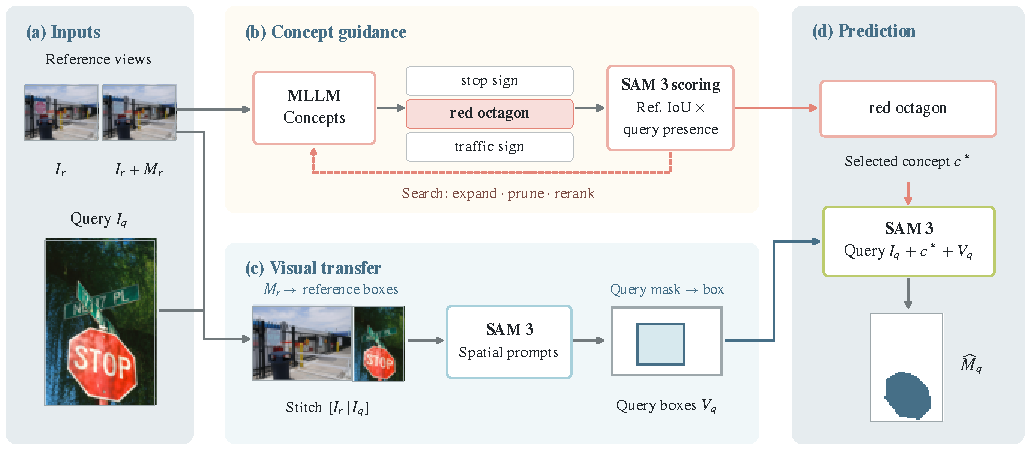
\includegraphics[width=\linewidth]{figures/cgics_pipeline.pdf}
    \caption{\textbf{CG-ICS: concept guidance.} Concept search and visual transfer supply text and box prompts for the final SAM~3 query segmentation; the box icon is schematic.}
    \label{fig:cgics}
\end{figure*}

The visual branch concatenates the reference and query. Reference-mask components provide spatial prompts on this combined image; the resulting query-side masks yield box prompts. SAM~3 then combines these boxes with the selected concept to segment the query (Figure~\ref{fig:cgics}). We compare a single concept, scored candidates, and full search, each with and without visual boxes. Visual-only and direct-concatenation outputs provide additional controls.

The implemented system uses Qwen3-VL-4B-Instruct for concept generation~\cite{qwen3vl}, working image size 512, five initial candidates, and three search loops. SAM~3 applies its own size-1008 preprocessing. The language model and segmenter occupy separate GPUs; this additional language-model allocation is included when interpreting system cost.
